\documentclass[a4paper, 12pt]{article}

\usepackage[portuges]{babel}
\usepackage[utf8]{inputenc}
\usepackage[margin=1.2in]{geometry}
\usepackage{amsmath}
\usepackage{graphicx}
\usepackage{datetime}
\usepackage{enumerate}
\usepackage{float}
\renewcommand{\baselinestretch}{1.5}

\emergencystretch 1pt%
\setlength{\parindent}{0pt}

\title{EFC3 - MLP e SVM}
\author{Rafael Gonçalves - RA: 186062}

\begin{document}


\maketitle

\section*{Parte I - Retropropagação de erro}

A rede apresentada pode ser descrita como:

\begin{equation}
    \mathbf{y} = \sum\mathbf{W}\mathbf{F}\left (\sum\mathbf{V}\mathbf{x}\right )
\end{equation}

em que $\mathbf{y}$ é o vetor de saídas, $\mathbf{x}$ é o vetor de entradas incluindo um valor unitário para facilitar o cálculo do bias, $V$ e $W$ são as matrizes de peso e $\mathbf{F}(\mathbf{x})$ uma matriz diagonal com os únicos elementos não nulos sendo $\mathbf{F_{i,i}}(\mathbf{x}) = f(x_i)$

Podemos definir $\mathbf{u} = \sum\mathbf{Vx}$ e $\mathbf{a} = \mathbf{F}(\mathbf{u})$ para facilitar os cálculos do gradiente.

A função de custo é:

\begin{equation}
    J = \mathbf{e^Te}
\end{equation}

Com $\mathbf{e} = {\mathbf{y_{target}} - \mathbf{y}}$, $\mathbf{y}$ sendo o vetor coluna que representa a saída da rede e $\mathbf{y_{target}}$ o vetor coluna com os rótulos.

Então o cálculo do gradiente se dá da seguinte forma:

\[
    \frac{\partial J}{\partial \mathbf{W}} = \frac{\partial J}{\partial \mathbf{e}}\frac{\partial\mathbf{e}}{\partial\mathbf{y}}\frac{\partial\mathbf{y}}{\partial\mathbf{W}} = 2\mathbf{e}(-1)\mathbf{a} = \boldsymbol{\delta _W} \mathbf{a}
\]

\[
    \frac{\partial J}{\partial \mathbf{V}} = \frac{\partial J}{\partial \mathbf{e}}\frac{\partial\mathbf{e}}{\partial\mathbf{y}}\frac{\partial\mathbf{y}}{\partial\mathbf{a}}\frac{\partial\mathbf{a}}{\partial\mathbf{u}}\frac{\partial\mathbf{u}}{\partial\mathbf{V}} = 2\mathbf{e}(-1)\mathbf{W}\mathbf{\dot{F}}(\mathbf{u})\mathbf{x} = \boldsymbol{\delta _V} \mathbf{x}
\] 

\vspace{1em}
em que $\dot{\mathbf{F}}_{i,j}(\mathbf{u}) = \dot{f}(u_i)$ se $i = j$ e vale $0$ caso o contrário.

Desta maneira podemos calcular:

\[
    \frac{\partial J}{\partial v_{21}} = -2e_1w_{20}\dot{f}(u_1 ) x_2 - 2e_2w_{21}\dot{f}(u_1) x_2
\]

\vspace{1em}
em que $u_1 = v_{01} + v_{11}x_1 + v_{12}x_2$ e $e_1 = {y_{target}}_1 - y_1$

\section*{Parte II - Classificação binária com MLPs e SVMs}

\subsection*{Multilayer Perceptrons}

O modelo utilizado foi uma rede neural de 2 camadas implementada usando a biblioteca pytorch que consistem em:
\begin{enumerate}
\item
    Camada intermediária com 30 neurônios e com a função linear como função de ativação (ReLU)
\item
    Camada de saída com 1 neurônio e com função logística como função de ativação 
\end{enumerate}

A função de custo utilizada foi a entropia cruzada.
Para calcular os parâmetros foi usado o método Adam, que apresentou uma convergência mais rápida do que com o método de gradiente descendente estocástico.

A acurácia no conjunto de teste foi de 88,3\% (erro = 11,7\%)

Os parâmetros foram escolhidos usando a técnica de validação cruzada (holdout) no conjunto de validação com os valores 3, 6, 10, 30, 60 como opções para o número de neurônios na camada intermediária. Ambas redes com 30 e 60 neurônios obtiveram a mesma acurácia para o conjunto de validação, portanto foi escolhido o modelo mais simples (30 neurônios).

Também foi testado o aprendizado tanto padrão-a-padrão como batelada (este último utilizando a técnica de drop-out para minimizar overfitting) e a primeira técnica foi a que obteve uma acurácia maior.

\begin{figure}[H]
    \centering
  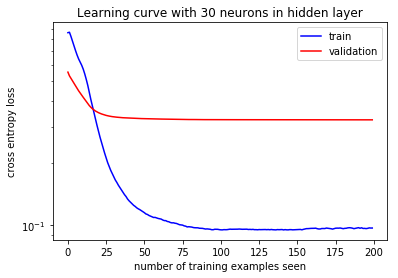
\includegraphics[width=9cm]{images/online_curve_h_30.png}
    \caption{Curva de aprendizado do modelo descrito. O eixo y mostra em escala logarítimica o valor da função de custo e o eixo x mostra o número de épocas passadas.}
\end{figure}



Análisando a figura 1 podemos perceber que o modelo melhora consideravelmente nas primeiras 50 iterações, depois tende a se estabilizar o valor no conjunto de validação e apenas melhora o custo em relação ao conjunto de treino. Isso se dá pois o modelo é capaz de extrair toda informação dos dados de treino e depois disso começa a aprender no sentido de memorizar os dados exatos de treino (overfitting).

\begin{figure}[H]
\centering
\begin{minipage}{.5\textwidth}
  \centering
  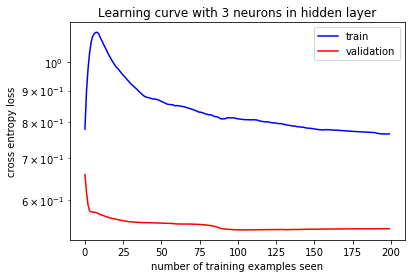
\includegraphics[width=.9\linewidth]{images/online_curve_h_3.png}
  % \captionof{figure}{A figure}
  % \label{fig:test1}
\end{minipage}%
\begin{minipage}{.5\linewidth}
  \centering
  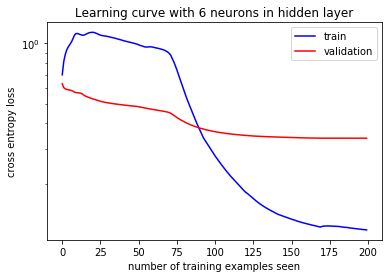
\includegraphics[width=.9\linewidth]{images/online_curve_h_6.png}
  % \captionof{figure}{Another figure}
  % \label{fig:test2}
\end{minipage}
    \caption{Curva de aprendizado para rede com 3 (esquerda) e 6 (direita) neurônios na camada intermediária.}
\end{figure}

Os modelos com menos neurônios (figura 2) alcançaram medidas menores para acurácia (portanto maiores para erro) e maiores para o custo, mostrando que a capacidade do modelo seria insuficiente para ser escolhido como bom modelo para ser usado no problema.

\begin{figure}[H]
    \centering
  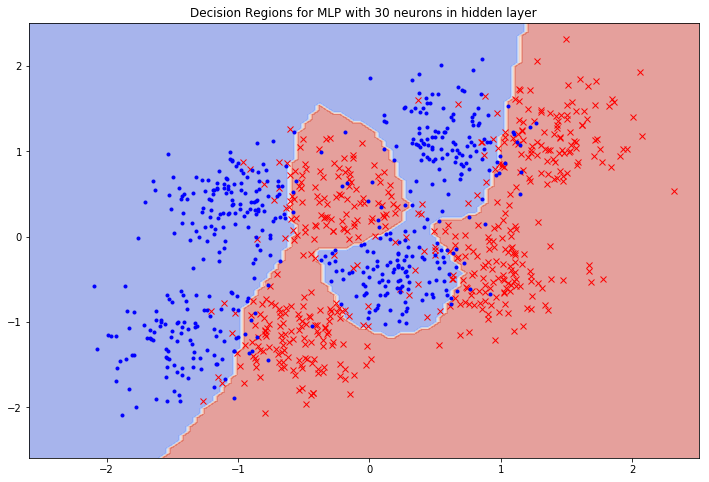
\includegraphics[width=15cm]{images/mlp_regions_h_30.png}
    \caption{Regiões de decisão mapeadas pela rede. Também está mostrado a classe real de cada uma das entradas do conjunto de teste.}
\end{figure}

Analisando a figura 3 podemos ver as áreas que o modelo mapeia para cada classe que é bastante similar ao resultado apresentado pelo estimador MAP. Na mesma figura podemos ver os dados do conjunto de teste com seus respectivos rótulos. É possível perceber que os pontos que foram classificados de forma errada são os pontos que estão muito próximos de uma densidade mais elevada de pontos da outra classe.

\subsection*{Support-vector Machines}

Par as máquinas de vetores-suporte, foi usado o modelo da biblioteca sci-kit learn. Os hiperparâmetros também foram escolhidos por holdout.
O modelo final escolhido foi um SVM com kernel rbf e C = 50

A acurácia do modelo foi de 87,6\% (erro de 12,4\%).

\begin{figure}[H]
    \centering
  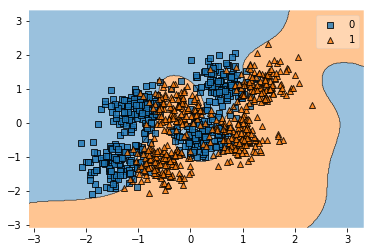
\includegraphics[width=10cm]{images/test_regions_svm_50_rbf.png}
    \caption{Regiões de decisão mapeadas pelo SVM. Também está mostrado a classe real de cada uma das entradas do conjunto de teste.}
\end{figure}

Analisando a figura 4 é possível perceber regiões também parecidas com as da MLP. É interessante notar que onde não há dados o modelo faz um mapeamento mesmo assim que, por não ter influência no cálculo do custo, parece não ter a ver com os dados que foram apresentados.


Os vetores-suporte não foram plotados, mas ficou claro que são diretamente influenciados pelo hiperparâmetro de penalização C. Quanto maior o valor de C, menos são os vetores-suporte.

Alguns outros modelos gerados variando o valor de C e o kernel:

\begin{figure}[H]
    \centering
  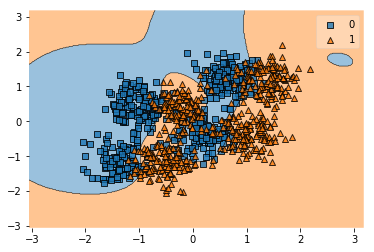
\includegraphics[width=8cm]{images/regions_svm_1_rbf.png}
    \caption{Regiões de decisão mapeadas pelo SVM com C = 1 e kernel rbf. Acurácia 85\%, 521 vetores-suporte.}
\end{figure}

\begin{figure}[H]
    \centering
  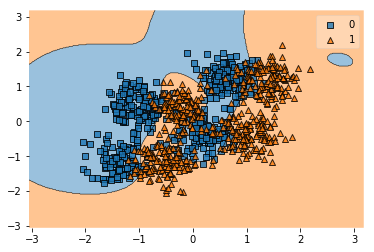
\includegraphics[width=8cm]{images/regions_svm_100_rbf.png}
    \caption{Regiões de decisão mapeadas pelo SVM com C = 100 e kernel rbf. Acurácia 86\%, 289 vetores-suporte.}
\end{figure}

\begin{figure}[H]
    \centering
  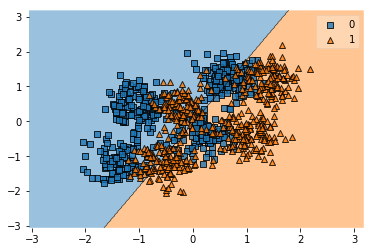
\includegraphics[width=8cm]{images/regions_svm_50_linear.png}
    \caption{Regiões de decisão mapeadas pelo SVM com C = 50 e kernel linear. Acurácia 66\%, 657 vetores-suporte.}
\end{figure}

Com o kernel linear (Figura 7), o SVM se comporta como um classificador linear, e portanto não tem a complexidade necessária para classificar o problema apresentado.

As figuras 5 e 6 mostram 2 valores diferentes para C com o mesmo kernel rbf. É possível perceber que com um valor baixo de C (ou seja, mais vetores-suporte sendo usados) a região mapeada parece se moldar de forma mais suave se comparada com um valor elevado de C.

\end{document}
